\documentclass[14pt,a4paper,fleqn]{extarticle}
\usepackage[T2A,T1]{fontenc}
\usepackage[utf8]{inputenc}
\usepackage[russian]{babel}
\usepackage{amsmath}
\usepackage{graphicx}
\usepackage{tabularx}
\usepackage{boldline}
\usepackage{makecell}
\usepackage{arydshln}
\usepackage{mathtools}

\graphicspath{ {./images/} }
\setlength{\mathindent}{0pt}
\setlength\parindent{0pt}


\begin{document}
	\begin{titlepage}
		
\includegraphics[scale=0.12]{logo}
		\begin{center}
			\textbf{МИНОБРНАУКИ РОССИИ}\\
			\vspace{0.2cm}
			\textbf{Федеральное государственное бюджетное образовательное учреждение высшего образования}\\
			\textbf{«САНКТ-ПЕТЕРБУРГСКИЙ ГОСУДАРСТВЕННЫЙ ЭКОНОМИЧЕСКИЙ УНИВЕРСИТЕТ»}\\
			\vspace{0.6cm}
			Факультет информатики и прикладной математики\\
			Кафедра прикладной математики и экономико-математических методов\\
			\vspace{1cm}
			\textbf{ОТЧЁТ}\\
			по дисциплине:\\
			\textbf{«Методы оптимизации»}\\
			на тему:\\
			\textbf{«Решение транспортной задачи. Задание 8»}\\
		\end{center}
		\vspace{1cm}
		Направление: 01.03.02\\
		Обучающийся: Бронников Егор Игоревич\\
		Группа: ПМ-1901\\
		\vfill
		\begin{center}
			Санкт-Петербург\\
			2021\\
		\end{center}
	\end{titlepage}
\section*{Задание 1. Сбалансированная задача}
\subsection*{Дано}
\begin{center}
	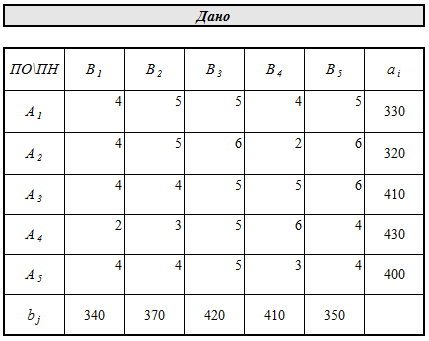
\includegraphics[scale=0.75]{1}
\end{center}
\newpage
\subsection*{a. Метод северо-западного угла}
\begin{center}
	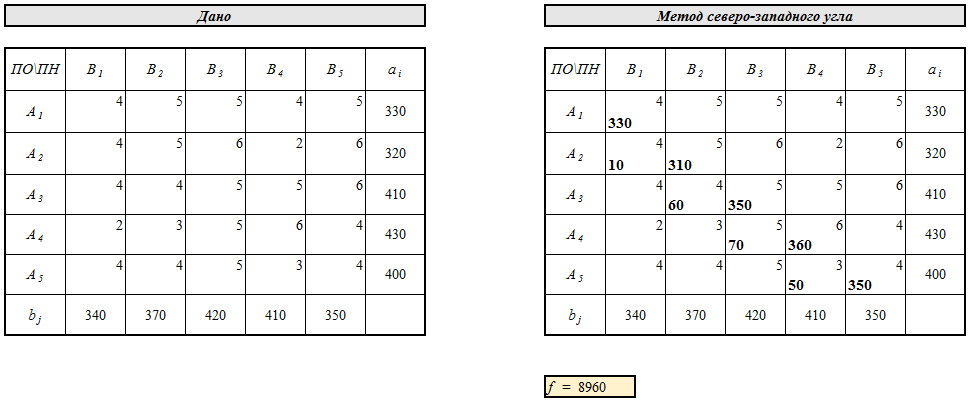
\includegraphics[scale=0.51]{2}
\end{center}
\small Рассматриваем левый верхний угол и ставим туда максимально возможную перевозку -- 330. Далее переходим ко второй строке и видим, что мы не выполнили все заказы в пункте $B_1$, поэтому дополняем пункт нужным количеством груза -- 10 и переходим к следующему пункту $B_2$. Тоже заполняем его максимально возможной перевозкой -- 310 и т. д.\\\\
\small $f = 4*330+4*10+5*310+4*60+5*350+5*70+6*360+3*50+4*350 = 8960$
\begin{center}
$\downarrow$
\end{center}
$f = 8960$\\\\
Стоит также отметить, что мы получили невырожденный допустимый план, так как количество базисных клеток совпало с $M+N-1 = 5+5-1 = 9$.
\newpage
\subsection*{b. Метод минимального элемента}
\begin{center}
	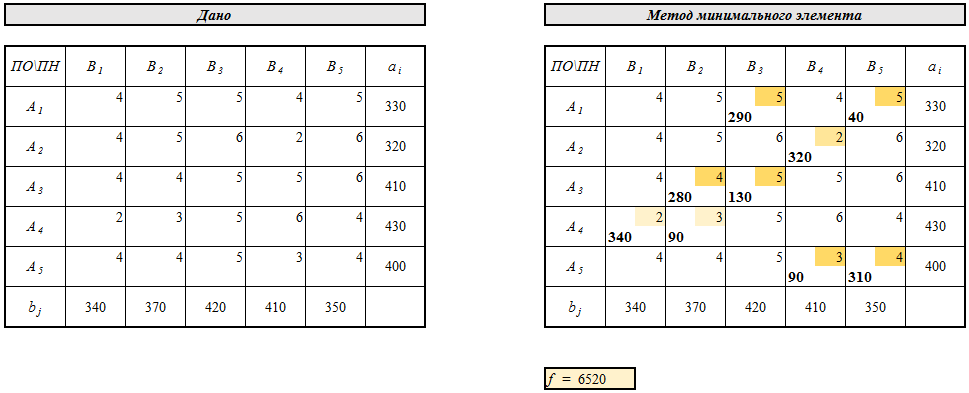
\includegraphics[scale=0.51]{3}
\end{center}
Находим минимальный тариф, в данном случае я выбрал $A_4B_1$ -- 2. В эту клетку записываем максимально возможную перевозку -- 340 и исключаем столбец $B_1$ из дальнейшего рассмотрения, так как мы удовлетворили данный пункт и т.д.\\\\
\small $f = 5*290+5*40+2*320+4*280+5*130+2*340+3*90+3*90+4*310 = 6520$
\begin{center}
	$\downarrow$
\end{center}
$f = 6520$\\\\
Стоит также отметить, что мы получили невырожденный допустимый план, так как количество базисных клеток совпало с $M+N-1 = 5+5-1 = 9$.
\newpage
\subsection*{c. Метод Фогеля}
\begin{center}
	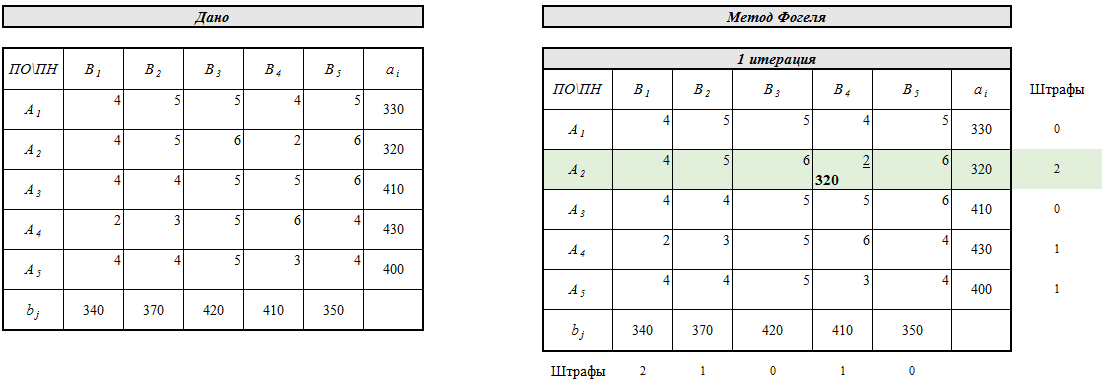
\includegraphics[scale=0.45]{4}
\end{center}
Сначала вычислим штрафы. Наибольший по строкам штраф получился 2, поэтому мы рассматриваем соответствующую строку -- 2. Далее в этой строке у нас минимальный тариф 2 и мы ему приписываем максимально возможную перевозку, то есть 320 и исключаем эту строку из рассмотрения. Переходим к следующему шагу.
\begin{center}
	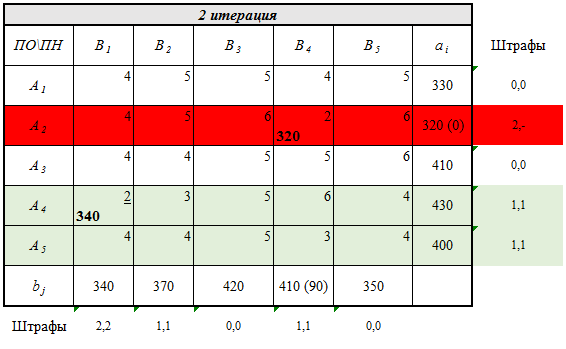
\includegraphics[scale=0.7]{5}
\end{center}
\newpage
\begin{center}
	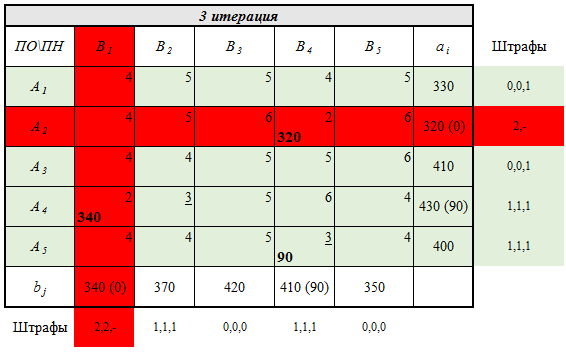
\includegraphics[scale=0.7]{6}
\end{center}
$\newline\newline$
\begin{center}
	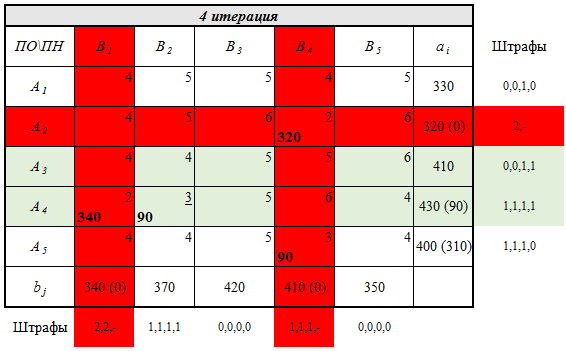
\includegraphics[scale=0.7]{7}
\end{center}
\newpage
\begin{center}
	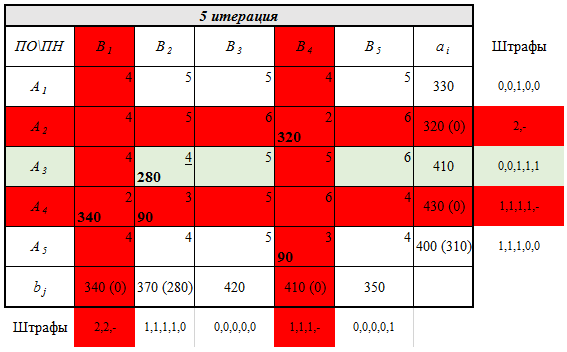
\includegraphics[scale=0.7]{8}
\end{center}
$\newline\newline$
\begin{center}
	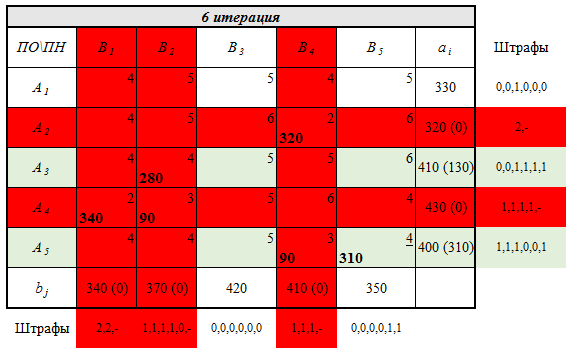
\includegraphics[scale=0.7]{9}
\end{center}
\newpage
\begin{center}
	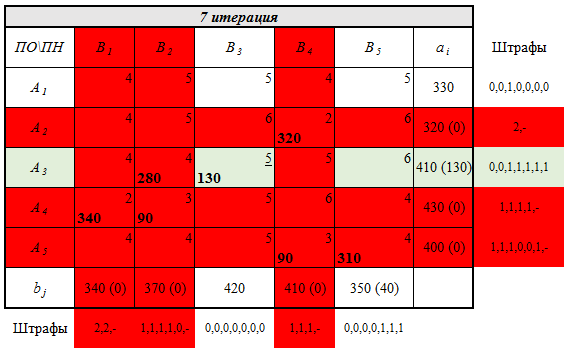
\includegraphics[scale=0.7]{10}
\end{center}
$\newline\newline$
\begin{center}
	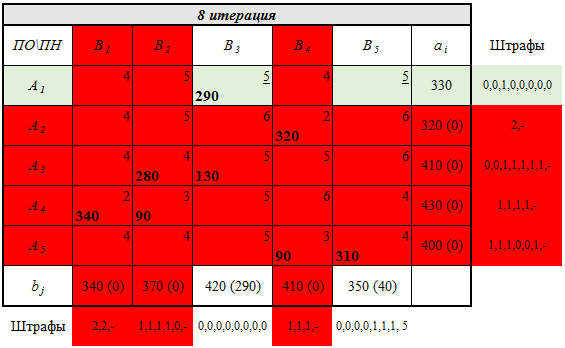
\includegraphics[scale=0.7]{11}
\end{center}
\newpage
\begin{center}
	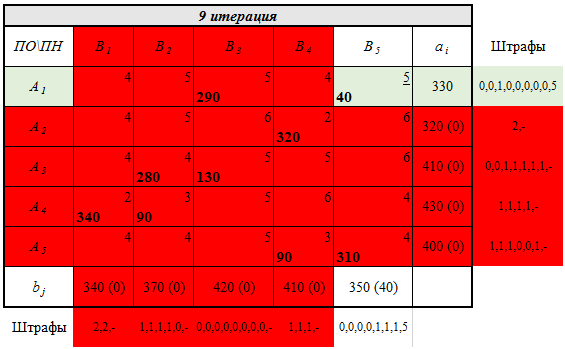
\includegraphics[scale=0.6]{12}
\end{center}
\begin{center}
	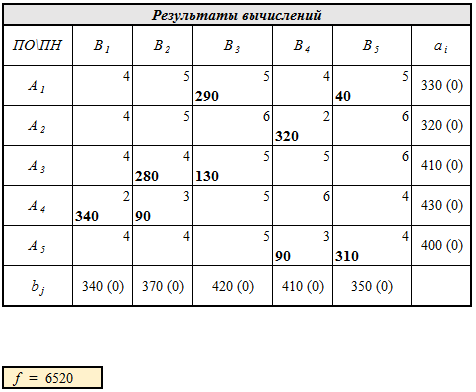
\includegraphics[scale=0.6]{13}
\end{center}
После 9 итериций мы получили следущий результат.\\
\small $f = 5*290 + 5*40 + 2*320 + 5*130 + 4*280 + 3*90 + 2*340 + 3*90 + 4*310 = 6520$
\begin{center}
$\downarrow$
\end{center}
$f = 6520$\\\\
Стоит также отметить, что мы получили невырожденный допустимый план, так как количество базисных клеток совпало с $M+N-1 = 5+5-1 = 9$.
\newpage
\subsection*{d. Метод потенциалов}
\begin{center}
	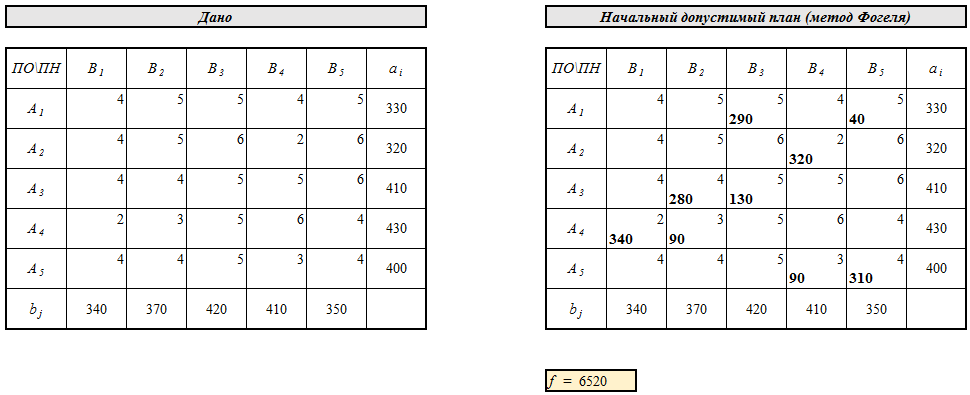
\includegraphics[scale=0.5]{14}
\end{center}
\begin{center}
	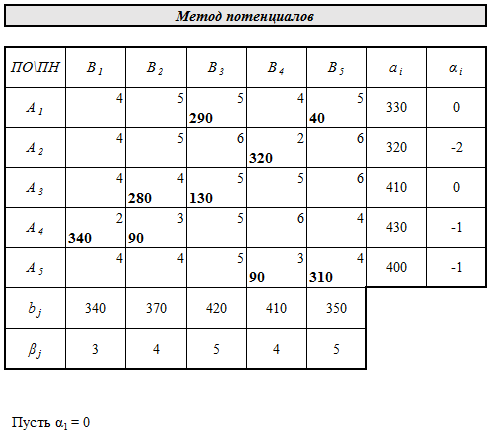
\includegraphics[scale=0.5]{15}
\end{center}
Проверим, является ли наш допустимый план оптимальным. Пусть $\alpha_1 = 0$, тогда мы получим соответствующие значения для платежей $\alpha_i$ и $\beta_j$.\\
$\alpha_1 + \beta_1 = 3 \leq 4 \hspace*{0.1cm} (c_{11}) \hspace*{1cm} \alpha_1 + \beta_2 = 4 \leq 5 \hspace*{0.1cm} (c_{12}) \hspace*{1cm} \alpha_1 + \beta_4 = 4 \leq 4 \hspace*{0.1cm} (c_{14})$\\
$\alpha_2 + \beta_1 = 1 \leq 4 \hspace*{0.1cm} (c_{21}) \hspace*{1cm} \alpha_2 + \beta_2 = 2 \leq 5 \hspace*{0.1cm} (c_{22}) \hspace*{1cm} \alpha_2 + \beta_3 = 3 \leq 6 \hspace*{0.1cm} (c_{23})$\\
$\alpha_2 + \beta_5 = 3 \leq 6 \hspace*{0.1cm} (c_{25}) \hspace*{1cm} \alpha_3 + \beta_1 = 3 \leq 4 \hspace*{0.1cm} (c_{31}) \hspace*{1cm} \alpha_3 + \beta_4 = 4 \leq 5 \hspace*{0.1cm} (c_{34})$\\
$\alpha_3 + \beta_5 = 5 \leq 6 \hspace*{0.1cm} (c_{35}) \hspace*{1cm} \alpha_4 + \beta_3 = 4 \leq 5 \hspace*{0.1cm} (c_{43}) \hspace*{1cm} \alpha_4 + \beta_4 = 3 \leq 6 \hspace*{0.1cm} (c_{44})$\\
$\alpha_4 + \beta_5 = 4 \leq 4 \hspace*{0.1cm} (c_{45}) \hspace*{1cm} \alpha_5 + \beta_1 = 2 \leq 4 \hspace*{0.1cm} (c_{51}) \hspace*{1cm} \alpha_5 + \beta_2 = 3 \leq 4 \hspace*{0.1cm} (c_{52})$\\
$\alpha_5 + \beta_3 = 4 \leq 5 \hspace*{0.1cm} (c_{53})$
\newpage
Получили, что во всех свободных клетках выполняется условие $c_{ij} \geq s_{ij}$, следовательно наш план является оптимальным.\\\\
Возьмём начальный план из метода северо-западного угла и сделаем 2 итерации.
\begin{center}
	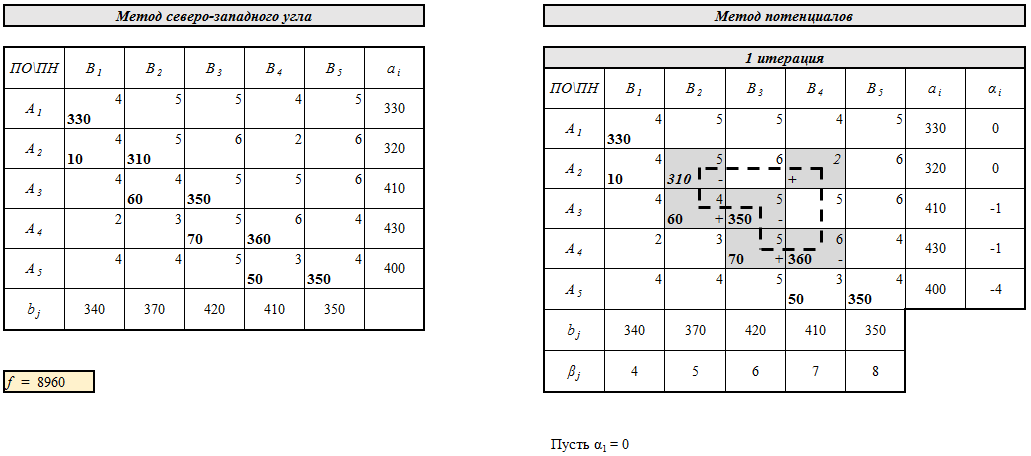
\includegraphics[scale=0.45]{16}
\end{center}
Пусть $\alpha_1 = 0$. Находим потенциалы $\alpha_i$ и $\beta_j$.\\
Проверим, будет ли являться наш план оптимальным:\\
$A_1B_2: 0 + 5 = 5 \leq 5$\\
$A_1B_3: 0 + 6= 6 > 5 \hspace*{0.3cm} \rightarrow v_{13} = 0 + 6 - 5 = 1$\\
$A_1B_4: 0 + 7 = 7 > 4 \hspace*{0.3cm} \rightarrow v_{14} = 0 + 7 - 4 = 3$\\
$A_1B_5: 0 + 8 = 8 > 5 \hspace*{0.3cm} \rightarrow v_{15} = 0 + 8 - 5 = 3$\\
$A_2B_3: 0 + 6 = 6 \leq 6$\\
$A_2B_4: 0 + 7 = 7 > 2 \hspace*{0.3cm} \rightarrow v_{24} = 0 + 7 - 2 = 5$\\
$A_2B_5: 0 + 8 = 8 > 6 \hspace*{0.3cm} \rightarrow v_{25} = 0 + 8 - 6 = 2$\\
$A_3B_1: -1 + 4 = 3 \leq 4$\\
$A_3B_4: -1 + 7 = 6 > 5 \rightarrow v_{34} = -1 + 7 - 6 = 1$\\
$A_3B_5: -1 + 8 = 7 > 6 \rightarrow v_{35} = -1 + 8 - 7 = 1$\\
$A_4B_1: -1 + 4 = 3 > 2 \rightarrow v_{41} = -1 + 4 - 3 = 1$\\
$A_4B_2: -1 + 5 = 4 > 3 \rightarrow v_{42} = -1 + 5 - 3 = 1$\\
$A_4B_5: -1 + 8 = 7 > 4 \rightarrow v_{45} = -1 + 8 - 4 = 3$\\
$A_5B_1: -4 + 4 = 0 \leq 4$\\
$A_5B_2: -4 + 5 = 1 \leq 4$\\
$A_5B_3: -4 + 6 = 2 \leq 5$\\\\
$max\hspace*{0.1cm}\{1,3,3,5,2,1,1,1,1,3\} = 5$
\newpage
Следовательно выбираем свободную клетку $A_2B_4$, так как она имеет максимальный штраф и строим из неё цикл.\\\\
Цикл: $A_2B_4 \rightarrow A_2B_2 \rightarrow A_3B_2 \rightarrow A_3B_3 \rightarrow A_4B_3 \rightarrow A_4B_4$\\\\
Максимальное количество груза, которое мы можем перебросить по этому циклу -- 310. Наша целевая функция изменится на следующее значение:\\\\
$\delta f = 310*[(2+4+5)-(5+5+6)] = -1550$\\\\
В результате после 1 итерации мы получаем следующий план:
\begin{center}
	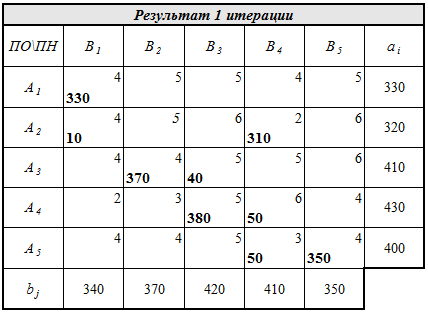
\includegraphics[scale=0.5]{17}
\end{center}
$A_2B_2$ стала свободной клеткой, а $A_2B_4$ стала базисной клеткой.\\
Переходим ко 2 итерации.\\
\begin{center}
	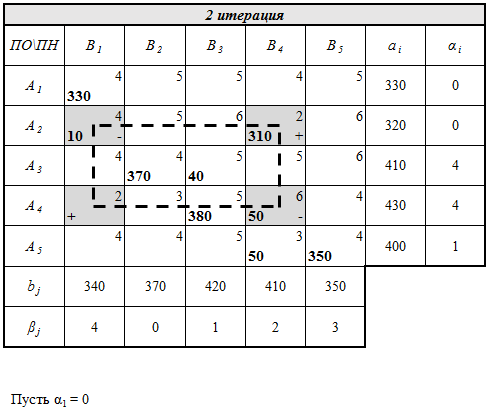
\includegraphics[scale=0.5]{18}
\end{center}
\newpage
Пусть $\alpha_1 = 0$. Находим потенциалы $\alpha_i$ и $\beta_j$.\\
Проверим, будет ли являться наш план оптимальным:\\
$A_1B_2: 0 + 0 = 0 \leq 5$\\
$A_1B_3: 0 + 1 = 1 \leq 5$\\
$A_1B_3: 0 + 2 = 2 \leq 4$\\
$A_1B_4: 0 + 2 = 2 \leq 4$\\
$A_1B_5: 0 + 3 = 3 \leq 4$\\
$A_2B_2: 0 + 0 = 0 \leq 5$\\
$A_2B_3: 0 + 1 = 1 \leq 6$\\
$A_2B_5: 0 + 3 = 3 \leq 6$\\
$A_2B_5: 0 + 3 = 3 \leq 6$\\
$A_3B_1: 4 + 4 = 8 > 4 \rightarrow v_{31} = 4 + 4 - 4 = 4$\\
$A_3B_4: 4 + 2 = 6 > 5 \rightarrow v_{34} = 4 + 2 - 5 = 1$\\
$A_3B_5: 4 + 3 = 7 > 6 \rightarrow v_{34} = 4 + 3 - 6 = 1$\\
$A_4B_1: 4 + 4 = 8 > 2 \rightarrow v_{41} = 4 + 4 - 2 = 6$\\
$A_4B_2: 4 + 0 = 4 > 3 \rightarrow v_{42} = 4 + 0 - 3 = 1$\\
$A_4B_5: 4 + 3 = 7 > 4 \rightarrow v_{45} = 4 + 3 - 4 = 3$\\
$A_5B_1: 1 + 4 = 5 > 4 \rightarrow v_{51} = 4 + 1 - 4 = 1$\\
$A_5B_2: 1 + 0 = 1 \leq 4$\\
$A_5B_3: 1 + 1 = 2 \leq 5$\\\\
$max\hspace*{0.1cm}\{4,1,1,6,1,3,1\} = 6$\\\\
Следовательно выбираем свободную клетку $A_4B_1$, так как она имеет максимальный штраф и строим из неё цикл.\\\\
Цикл: $A_4B_1 \rightarrow A_4B_4 \rightarrow A_2B_4 \rightarrow A_2B_1$\\\\
Максимальное количество груза, которое мы можем перебросить по этому циклу -- 10. Наша целевая функция изменится на следующее значение:\\\\
$\delta f = 10*[(2+2)-(4+6)] = -60$
\newpage
В результате после 2 итерации мы получаем следующий план:
\begin{center}
	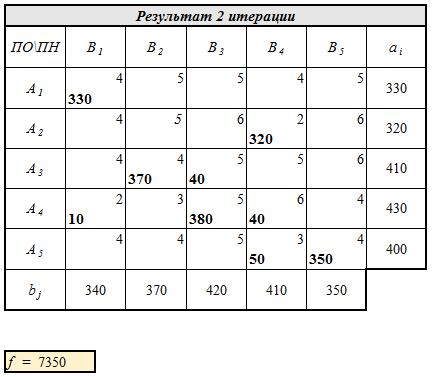
\includegraphics[scale=0.5]{19}
\end{center}
$A_2B_1$ стала свободной клеткой, а $A_4B_1$ стала базисной клеткой.\\
Значение целевой функции после двух итераций стало:\\\\
$f = 8960-(1550+60) = 7350$
\newpage
\section*{Задание 2. Несбалансированная задача}
\subsection*{Дано}
\begin{center}
	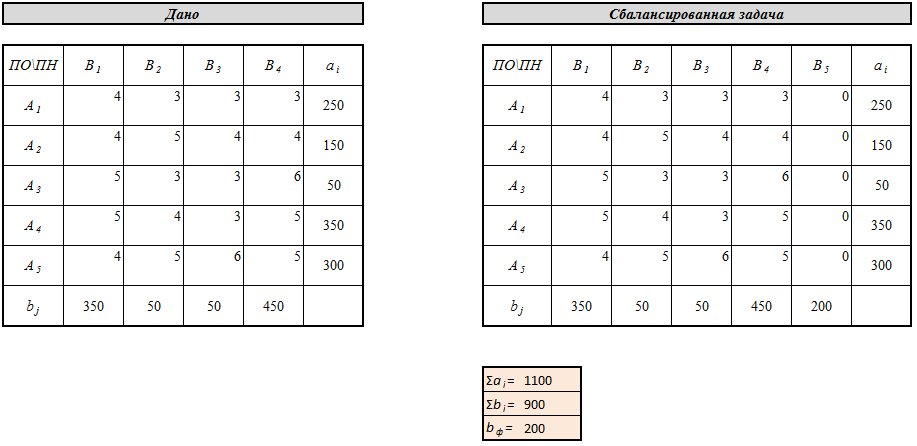
\includegraphics[scale=0.5]{20}
\end{center}
У нас получается несбалансированная задача, так как:\\
$\smashoperator[r]{\sum_{i=1}^{5}} a_i = 250+150+50+350+300 = 1100$\\\\
$\smashoperator[r]{\sum_{j=1}^{4}} b_j = 350+50+50+450 = 900$\\\\
А именно траспортная задача с избытком запасов, так как: $\smashoperator[r]{\sum_{i=1}^{5}} a_i > \smashoperator[r]{\sum_{j=1}^{4}} b_j$\\\\
Вводим фиктивный пункт $B_5$ с количеством заявок: $b_f = 1100 - 900 = 200$. Цены перевозок задаём равными нулю: $c_{fj} = 0, \hspace*{0.3cm} j = 1,...,5$. В итоге мы получили сбалансированную задачу.
\newpage
\subsection*{a. Метод северо-западного угла}
\begin{center}
	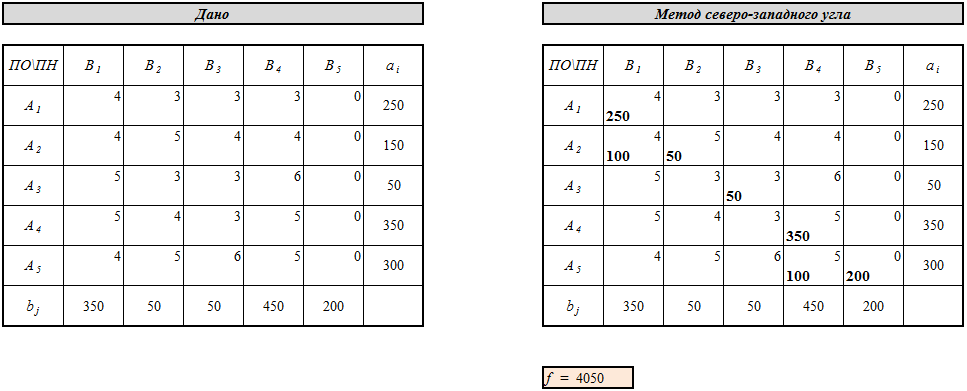
\includegraphics[scale=0.51]{21}
\end{center}
Алгоритм такой же как и в прошлом задании.\\\\
\small $f = 4*250+4*100+5*50+3*50+5*350+5*100+0*200 = 4050$
\begin{center}
	$\downarrow$
\end{center}
$f = 4050$\\\\
Стоит также отметить, что мы получили вырожденный допустимый план, так как количество базисных клеток не совпало с $M+N-1 = 5+5-1 = 9$, а базисных клеток у нас 7.
\newpage
Сведём этот план к невырожденному. Сделаем так, чтобы базисные клетки можно было бы соединить ломанной линией. В итоге получаем следующий результат:\\
\begin{center}
	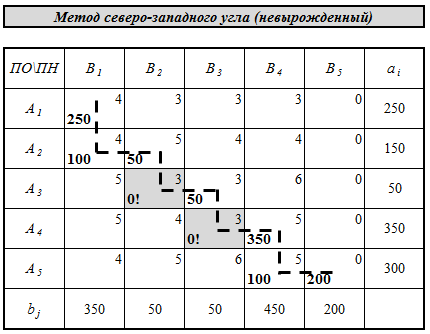
\includegraphics[scale=0.6]{22}
\end{center}
То есть клетки $A_3B_2$ и $A_4B_3$ мы сделали базисными с перевозкой 0.
\newpage
\subsection*{b. Метод минимального элемента}
\begin{center}
	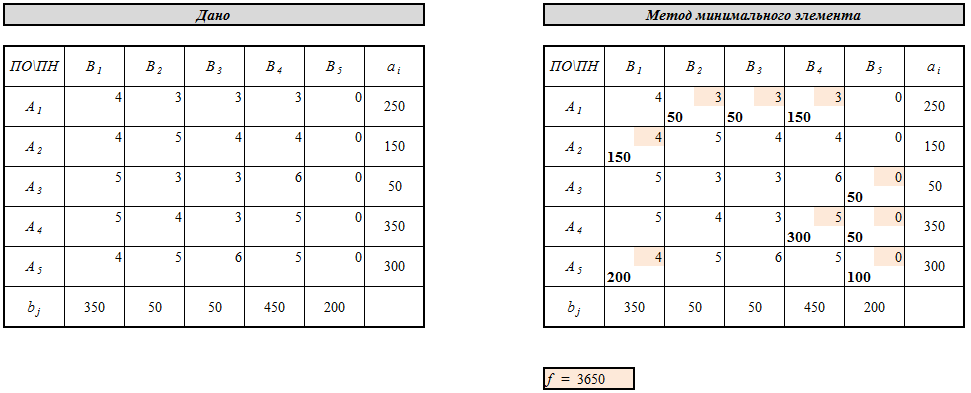
\includegraphics[scale=0.51]{23}
\end{center}
Алгоритм такой же как и в прошлом задании.\\\\
\small $f = 3*50+3*50+3*150+4*150+0*50+5*300+0*50+4*200+0*100 = 3650$
\begin{center}
	$\downarrow$
\end{center}
$f = 3650$\\\\
Стоит также отметить, что мы получили невырожденный допустимый план, так как количество базисных клеток совпало с $M+N-1 = 5+5-1 = 9$.
\newpage
\subsection*{c. Метод Фогеля}
\begin{center}
	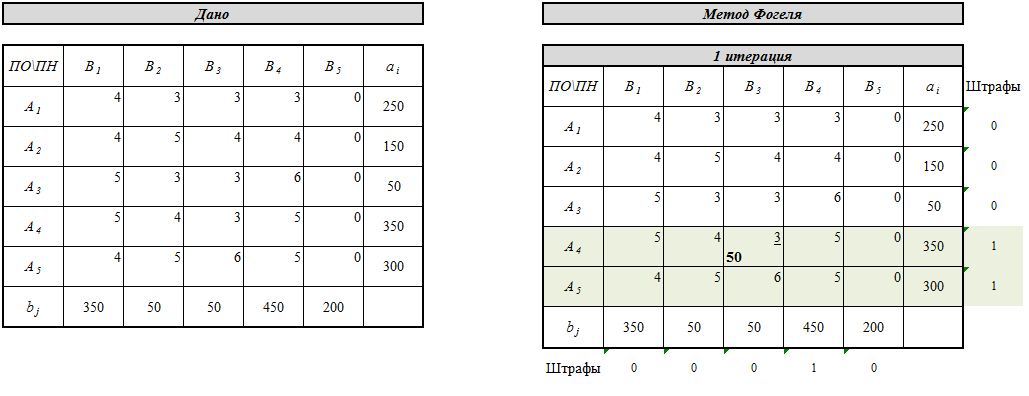
\includegraphics[scale=0.45]{24}
\end{center}
Алгоритм такой же как и в прошлом задании.\\
\begin{center}
	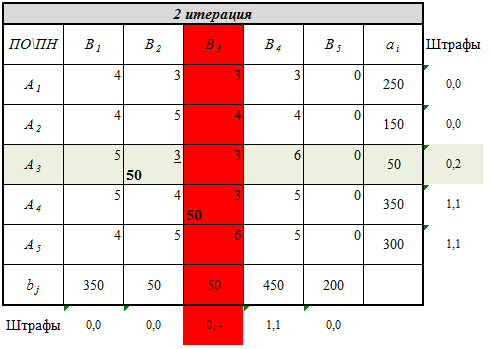
\includegraphics[scale=0.7]{25}
\end{center}
\newpage
\begin{center}
	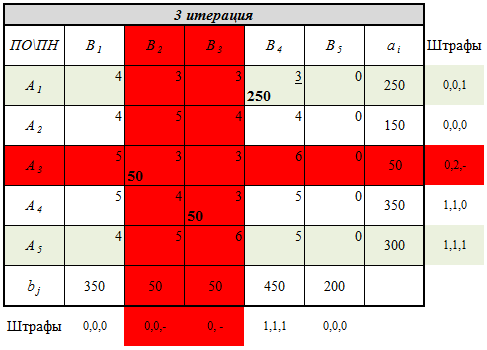
\includegraphics[scale=0.7]{26}
\end{center}
$\newline\newline$
\begin{center}
	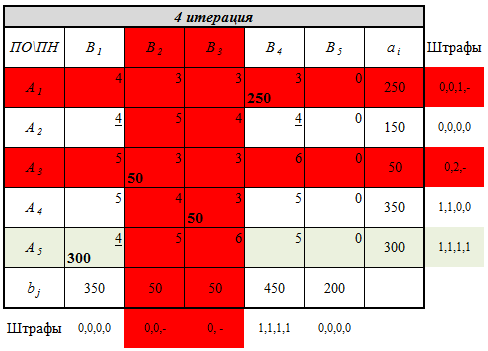
\includegraphics[scale=0.7]{27}
\end{center}
\newpage
\begin{center}
	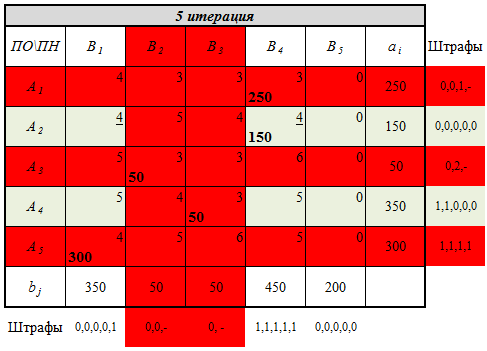
\includegraphics[scale=0.7]{28}
\end{center}
$\newline\newline$
\begin{center}
	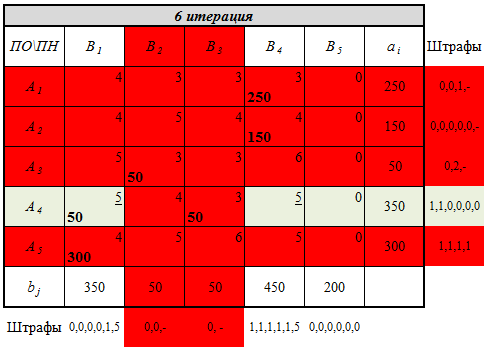
\includegraphics[scale=0.7]{29}
\end{center}
\newpage
\begin{center}
	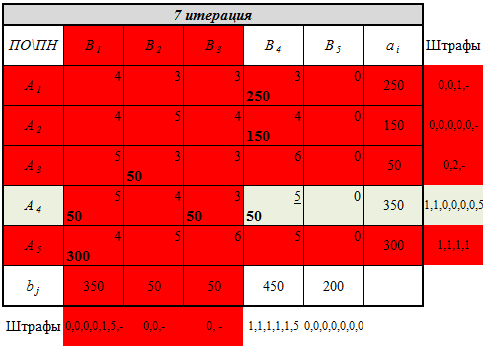
\includegraphics[scale=0.7]{30}
\end{center}
$\newline\newline$
\begin{center}
	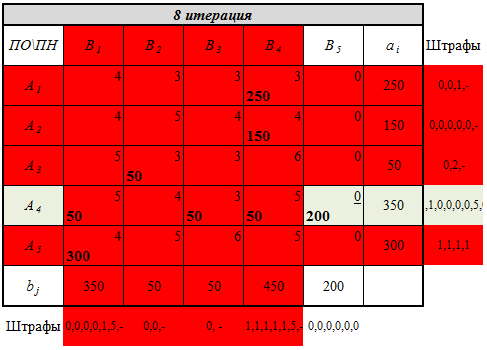
\includegraphics[scale=0.7]{31}
\end{center}
\newpage
После 8 итераций мы получили следующий результат:
\begin{center}
	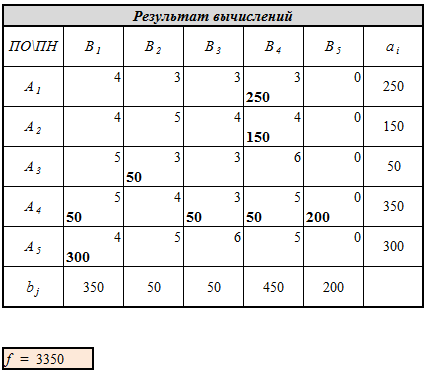
\includegraphics[scale=0.5]{32}
\end{center}
\small $f = 3*250+4*150+3*50+5*50+3*50+5*50+0*200+4*300 = 3350$
\begin{center}
	$\downarrow$
\end{center}
$f = 3350$\\\\
Стоит также отметить, что мы получили вырожденный допустимый план, так как количество базисных клеток не совпало с $M+N-1 = 5+5-1 = 9$, а базисных клеток у нас 8.
\newpage
Сведём этот план к невырожденному. В итоге получаем следующий результат:\\
\begin{center}
	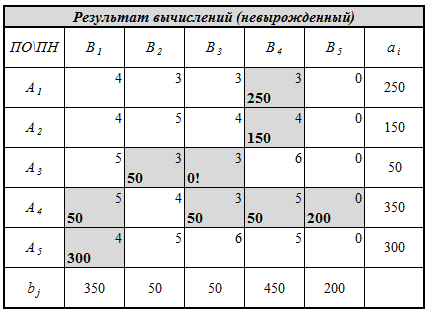
\includegraphics[scale=0.6]{33}
\end{center}
То есть клетку $A_3B_3$ мы сделали базисной с перевозкой 0.
\newpage
\subsection*{d. Метод потенциалов}
\begin{center}
	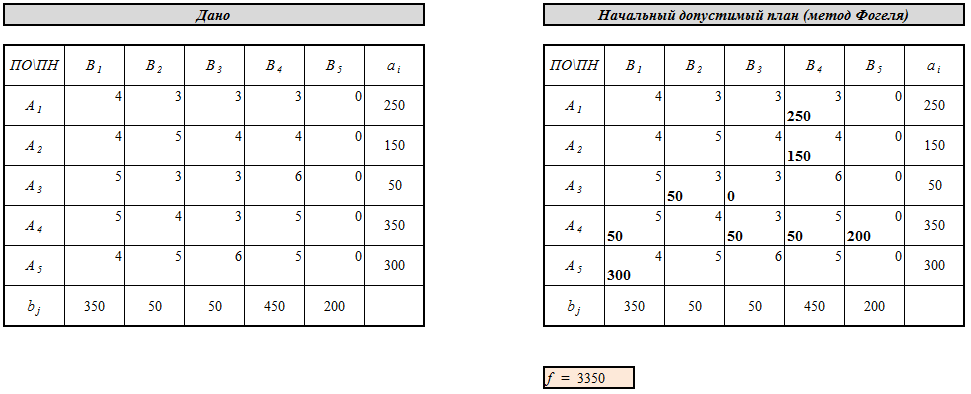
\includegraphics[scale=0.5]{34}
\end{center}
\begin{center}
	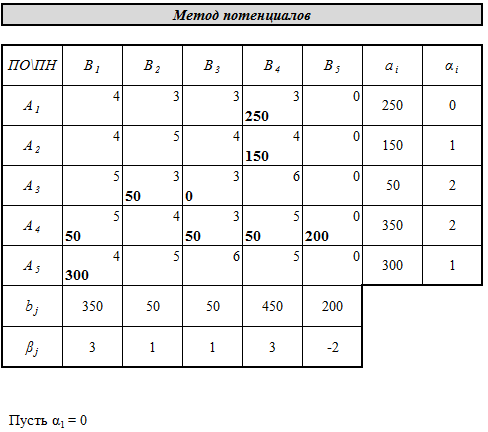
\includegraphics[scale=0.5]{35}
\end{center}
Проверим, является ли наш допустимый план оптимальным. Пусть $\alpha_1 = 0$, тогда мы получим соответствующие значения для платежей $\alpha_i$ и $\beta_j$.\\
$\alpha_1 + \beta_1 = 3 \leq 4 \hspace*{0.4cm} (c_{11}) \hspace*{1cm} \alpha_1 + \beta_2 = 1 \leq 3 \hspace*{0.4cm} (c_{12}) \hspace*{1cm} \alpha_1 + \beta_3 = 1 \leq 3 \hspace*{0.1cm} (c_{13})$\\
$\alpha_1 + \beta_5 = -2 \leq 0 \hspace*{0.1cm} (c_{15}) \hspace*{1cm} \alpha_2 + \beta_1 = 4 \leq 4 \hspace*{0.4cm} (c_{21}) \hspace*{1cm} \alpha_2 + \beta_2 = 2 \leq 5 \hspace*{0.1cm} (c_{22})$\\
$\alpha_2 + \beta_3 = 2 \leq 4 \hspace*{0.4cm} (c_{23}) \hspace*{1cm} \alpha_2 + \beta_5 = -1 \leq 0 \hspace*{0.1cm} (c_{25}) \hspace*{1cm} \alpha_3 + \beta_1 = 5 \leq 5 \hspace*{0.1cm} (c_{31})$\\
$\alpha_3 + \beta_4 = 5 \leq 6 \hspace*{0.4cm} (c_{34}) \hspace*{1cm} \alpha_3 + \beta_5 = 0 \leq 0 \hspace*{0.4cm} (c_{35}) \hspace*{1cm} \alpha_4 + \beta_2 = 3 \leq 4 \hspace*{0.1cm} (c_{42})$\\
$\alpha_5 + \beta_2 = 2 \leq 5 \hspace*{0.4cm} (c_{52}) \hspace*{1cm} \alpha_5 + \beta_3 = 2 \leq 6 \hspace*{0.4cm} (c_{53}) \hspace*{1cm} \alpha_5 + \beta_4 = 4 \leq 5 \hspace*{0.1cm} (c_{54})$\\
$\alpha_5 + \beta_5 = -1 \leq 0 \hspace*{0.1cm} (c_{55})$
\newpage
Получили, что во всех свободных клетках выполняется условие $c_{ij} \geq s_{ij}$, следовательно наш план является оптимальным.\\\\
Возьмём начальный план из метода северо-западного угла и сделаем 2 итерации.
\begin{center}
	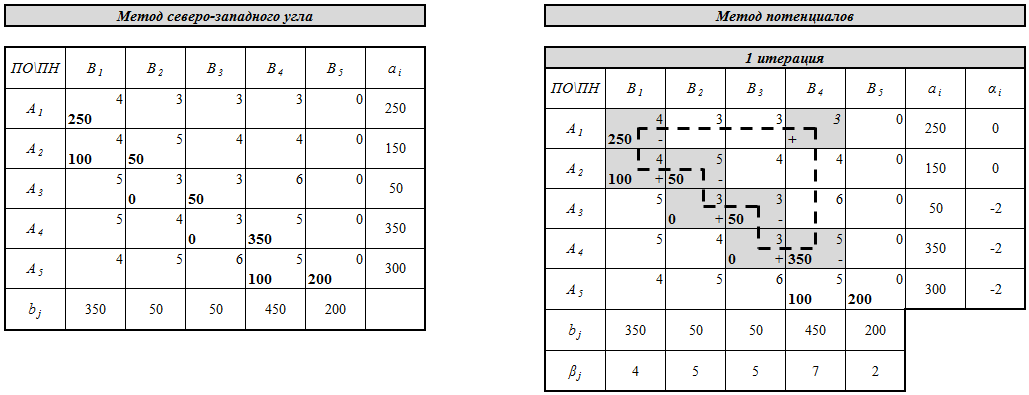
\includegraphics[scale=0.45]{36}
\end{center}
Пусть $\alpha_1 = 0$. Находим потенциалы $\alpha_i$ и $\beta_j$.\\
Проверим, будет ли являться наш план оптимальным:\\
$A_1B_2: 0 + 5 = 5 > 3 \hspace*{0.3cm} \rightarrow v_{12} = 0 + 5 - 3 = 2$\\
$A_1B_3: 0 + 5 = 5 > 3 \hspace*{0.3cm} \rightarrow v_{13} = 0 + 5 - 3 = 2$\\
$A_1B_4: 0 + 7 = 7 > 3 \hspace*{0.3cm} \rightarrow v_{14} = 0 + 7 - 3 = 4$\\
$A_1B_5: 0 + 2 = 2 > 0 \hspace*{0.3cm} \rightarrow v_{15} = 0 + 2 - 0 = 2$\\
$A_2B_3: 0 + 5 = 5 > 4 \hspace*{0.3cm} \rightarrow v_{23} = 0 + 5 - 4 = 1$\\
$A_2B_4: 0 + 7 = 7 > 4 \hspace*{0.3cm} \rightarrow v_{24} = 0 + 7 - 4 = 3$\\
$A_2B_5: 0 + 2 = 2 > 0 \hspace*{0.3cm} \rightarrow v_{25} = 0 + 2 - 0 = 2$\\
$A_3B_1: -2 + 4 = 2 \leq 5$\\
$A_3B_4: -2 + 7 = 5 \leq 6$\\
$A_3B_5: -2 + 2 = 0 \leq 0$\\
$A_4B_1: -2 + 4 = 2 \leq 5$\\
$A_4B_2: -2 + 5 = 3 \leq 4$\\
$A_4B_5: -2 + 2 = 0 \leq 0$\\
$A_5B_1: -2 + 4 = 2 \leq 4$\\
$A_5B_2: -2 + 5 = 3 \leq 5$\\
$A_5B_3: -2 + 5 = 3 \leq 6$\\\\
$max\hspace*{0.1cm}\{2,2,4,2,1,3,2\} = 4$
\newpage
Следовательно выбираем свободную клетку $A_1B_4$, так как она имеет максимальный штраф и строим из неё цикл.\\\\
Цикл: $A_1B_4 \rightarrow A_1B_1 \rightarrow A_2B_1 \rightarrow A_2B_2 \rightarrow A_3B_2 \rightarrow A_3B_3 \rightarrow A_4B_3 \rightarrow A_4B_4$\\\\
Максимальное количество груза, которое мы можем перебросить по этому циклу -- 50. Наша целевая функция изменится на следующее значение:\\\\
$\delta f = 50*[(3+4+3+3)-(4+5+3+5)] = -200$\\\\
В результате после 1 итерации мы получаем следующий план:
\begin{center}
	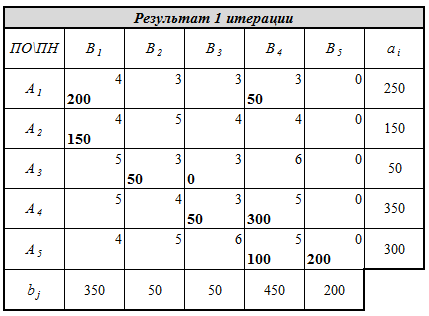
\includegraphics[scale=0.5]{37}
\end{center}
$A_2B_2$ стала свободной клеткой, а $A_1B_4$ стала базисной клеткой.\\
Переходим ко 2 итерации.\\
\begin{center}
	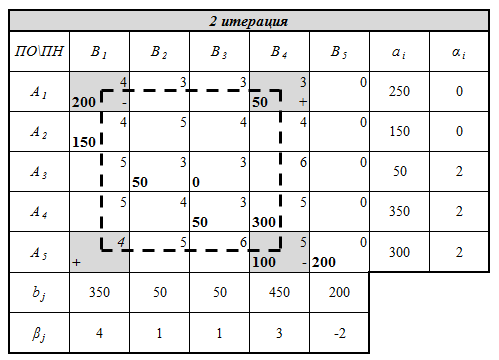
\includegraphics[scale=0.5]{38}
\end{center}
\newpage
Пусть $\alpha_1 = 0$. Находим потенциалы $\alpha_i$ и $\beta_j$.\\
Проверим, будет ли являться наш план оптимальным:\\
$A_1B_2: 0 + 1 = 1 \leq 3$\\
$A_1B_3: 0 + 1 = 1 \leq 3$\\
$A_1B_5: 0 - 2 = -2 \leq 0$\\
$A_2B_2: 0 + 1 = 1 \leq 5$\\
$A_2B_3: 0 + 1 = 1 \leq 4$\\
$A_2B_4: 0 + 3 = 3 \leq 4$\\
$A_2B_5: 0 - 2 = -2 \leq 0$\\
$A_3B_1: 2 + 4 = 6 > 5 \rightarrow v_{31} = 2 + 4 - 5 = 1$\\
$A_3B_4: 2 + 3 = 5 \leq 6$\\
$A_3B_5: 2 - 2 = 0 \leq 0$\\
$A_4B_1: 2 + 4 = 6 > 5 \rightarrow v_{41} = 2 + 4 - 5 = 1$\\
$A_4B_2: 2 + 1 = 3 \leq 4$\\
$A_4B_5: 2 - 2 = 0 \leq 0$\\
$A_5B_1: 2 + 4 = 6 > 4 \rightarrow v_{51} = 2 + 4 - 4 = 2$\\
$A_5B_2: 2 + 1 = 3 \leq 5$\\
$A_5B_3: 2 + 1 = 3 \leq 6$\\\\
$max\hspace*{0.1cm}\{1,1,2\} = 2$\\\\
Следовательно выбираем свободную клетку $A_5B_1$, так как она имеет максимальный штраф и строим из неё цикл.\\\\
Цикл: $A_5B_1 \rightarrow A_1B_1 \rightarrow A_1B_4 \rightarrow A_5B_4$\\\\
Максимальное количество груза, которое мы можем перебросить по этому циклу -- 100. Наша целевая функция изменится на следующее значение:\\\\
$\delta f = 100*[(3+4)-(4+5)] = -200$
\newpage
В результате после 2 итерации мы получаем следующий план:
\begin{center}
	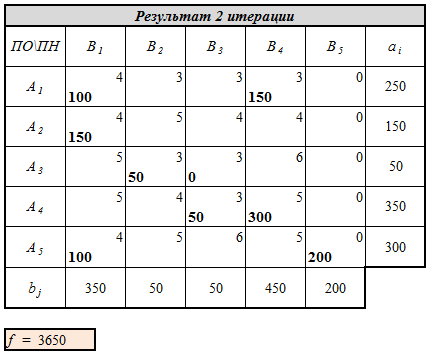
\includegraphics[scale=0.5]{39}
\end{center}
$A_5B_4$ стала свободной клеткой, а $A_5B_1$ стала базисной клеткой.\\
Значение целевой функции после двух итераций стало:\\\\
$f = 4050-(200+200) = 3650$
\end{document}